\documentclass[]{article}

\usepackage[utf8]{inputenc}

\usepackage{fullpage}
\usepackage{graphicx}
\graphicspath{{figures/}}
\usepackage[french]{babel}
\usepackage{url}
\usepackage[colorlinks=true, linkcolor=black]{hyperref}
\usepackage{color}
\usepackage[dvipsnames]{xcolor}
\usepackage{titling}
\usepackage{subfig}
\definecolor{mygray}{gray}{0.6}
\newcommand{\minit}[1]{\noindent{\small\textbf{ \underline{#1}}}\vspace{0.2cm}}


%-- Logos PDG --
\pretitle{
\begin{center}

\begin{figure}[!tbp]
  \centering
  \subfloat{
\includegraphics[width=0.25\textwidth]{UMons_logo.png}}
  \hfill
  \subfloat{
\includegraphics[width=0.25\textwidth]{sciences_logo.png}}\\
\end{figure}
~\newline

}

\posttitle{\end{center}}

\begin{document}

\title{
\vspace{1.6cm}
{\Huge Développement d'un pare-feu domestique}\\
\vspace{0.5cm}
{\Huge Pré-rapport de projet}\\
\vspace{0.2cm}
{\large Activité d' Apprentissage \textsf{S-INFO-037}}\\
}



\author{
\vspace{0.9cm}
\huge{Rémy Decocq}
}

\date{
\vspace{8.5cm}
Année Académique 2018-2019\\
Master en Sciences Informatiques, bloc 1\\
Faculté des Sciences, Université de Mons}

\maketitle          

\thispagestyle{empty}   

\newpage

\tableofcontents
\newpage

\section*{Introduction}

Depuis maintenant plusieurs décades, la connectique n'a cessé d'évoluer, que ce soit dans le cadre d'infrastructures de type "mainframe" ou dans le contexte des ordinateurs personnels. En conséquence, corrélé au fait de pouvoir de plus en plus s'interconnecter et rejoindre des réseaux de natures variées, le nombre de menaces potentielles pour une machine ainsi connectée augmente grandement. Heureusement, parallèlement à la connectique, les performances des machines classiques qui en sont équipée ont également suivi une bonne courbe de progression. Cela a permis d'en renforcer la sécurité à plusieurs niveaux, et surtout d'intercepter efficacement les menaces étrangères liées à l'utilisation des réseaux. À l'heure actuelle, les OS utilisés classiquement sur des machines desktop fournissent un pare-feu simple (\textit{Windows Defender}, un utilitaire fournit de base dans MAC OS X, \textit{iptables/Netfilter} ou autre pour les distributions Linux). Ce dernier tournant en arrière plan de façon quasi invisible car il demande peu de ressources par rapport à ce qu'une machine actuelle peut offrir.\\

\par En parallèle avec la montée en puissance de ces machines de type desktop, serveurs, etc. s'est développée depuis à peu près les années 2000 la tendance de l'\og Internet des Objets \fg{}, ou encore plus communément appelé IoT pour \textit{Internet of Things}. Assez complexe à définir, cette dénomination regroupe beaucoup d'objets et de concepts, qu'ils soient virtuels ou non : cela englobe notamment la domotique, les outils de mesures diverses connectés, les imprimantes et scanneurs en réseau, etc. Tous ces éléments tendent vers une mise en réseau commune, souvent directement avec l'Internet et un cloud permettant de traiter la masse de données qu'il reçoit de ces équipements. Or, comme évoqué ci-dessus, plus on s'interconnecte et plus on s'ouvre à des attaquants potentiels, ce qui pose problème si rien n'est mis en place pour s'en protéger.\\

\par Ce travail aura pour objectif premièrement de faire un état de l'art des dispositifs de protection qui sont actuellement déployés dans l'\textit{IoT} et globalement la sécurité dans ce \textit{Web 3.0}. Effectivement, on approche un monde beaucoup plus hétérogène et restreint en terme de ressources que celui des ordinateurs modernes et classiques, de fait on ne peut pas réutiliser telles quelles toutes les technologies de protection y attenant. Deuxièmement, il sera question de mettre en pratique ces connaissances pour développer un système en lien avec ces nouvelles mesures de sécurité inhérentes à l'\textit{IoT}, sous la forme d'un pare-feu.

\newpage
\section{Présentation de l'\textit{internet des objets}}

\subsection{Généralités}

\par L'Internet des objets, qu'on désignera par \textit{IoT} pour le terme plus répandu de \textit{Internet Of Things}, représente un tout qui évolue maintenant en flèche depuis plusieurs années. Aucune définition formelle n'est acceptée globalement, mais plusieurs organismes ont tenté d'en établir une ébauche. Par exemple, l'ITU-T (ITU Telecommunication Standardization Sector) Y.2060 le définit comme tel : 
\begin{center}
\textit{“Global  infrastructure  for  the  society,  enabling  advanced  services  by  inter-connecting (physical and virtual) things based on existing and evolving in-teroperable information and communication technologies.”}
\end{center}

\par Derrière cette définition très générale, on peut distinguer plusieurs sous-groupes d'objets connectés distincts, aux applications tant variées que hétérogènes, dans des domaines et secteurs également très différents. C'est ce qui fait la force et en même temps la faiblesse de ce tout ce qu'on regroupe derrière le terme \textit{IoT} et que des efforts considérables sont déployés pour inter-connecter au maximum. C'est un domaine d'étude intéressant car il représente littéralement ce qu'on pourrait considérer comme le futur de notre environnement technologique. De fait, les équipements que l'ont peut associer à une partie de l'IoT ont déjà fait leur apparition dans notre quotidien : en 2017 on comptait 8,4 milliards de machines en présentant les caractéristiques et les estimations pour l'année 2020 tendent vers 20,4 milliards d'objets connectés \cite{Berte2018}.  
\subsection{Caractéristiques des équipements de l'\textit{IoT}}

\subsubsection{Domaines d'application}

Les secteurs dans lesquels l'IoT s'est implanté ces dernières années sont nombreux et très variés : ils s'étendent de l'industrie au domaine des soins de santé en passant par la tendance des \textit{Smart Home}. C'est ce dernier domaine qui est approfondi dans ce travail et dont il sera le plus sous-entendu par la suite quand le terme \textit{IoT} est utilisé. La Figure~\ref{domains_IoT} présente une vision d'un schéma global des autres domaines qui gravitent autour du vaste monde de l'IoT.\\


\begin{figure}[!h]
\centering
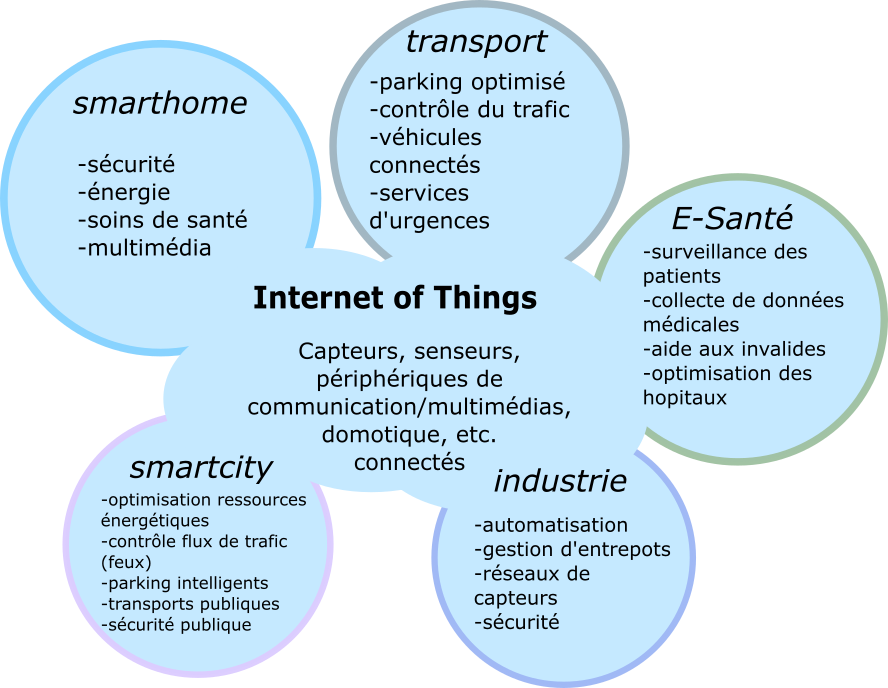
\includegraphics[width=0.6\linewidth]{IoT_domains.png}
\caption{Domaines d'application de l'IoT}
\label{domains_IoT}
\end{figure}

\newpage

\subsubsection{L'environnement \textit{smarthome}}
\par Le terme émergeant \textit{Smart Home} est une fois de plus très englobant et général, il n'en existe pas de définition formelle et validée de tous. Basman M. Hasan et al. \cite{Basman2016} en présente plusieurs, un résultat les unifiant pourrait être \textit{Une smarthome est un environnement lié au domicile particulier où plusieurs équipements ou sous-systèmes sont inter-connectés et où les informations qu'ils échangent sont collectées et utilisées afin de surveiller, réguler et automatiser l'écosystème du domicile.} L'utilisateur en tant que personne physique y vivant est donc au centre de cette architecture, et y siège comme le principal intervenant puisque dans l'idée où toute cette technologie est déployée dans le but d'améliorer sa qualité de vie, c'est lui qui devra interagir avec. La notion d'intelligence est intrinsèquement liée avec celle de l'interconnexion de tous ces senseurs et actuateurs déployés dans l'environnement du domicile : il s'agit d'en récolter et regrouper toutes les données en un point central doté d'une capacité de traitement plus évoluée afin qu'il puisse en tirer une optimisation globale du domicile et la proposer sous une forme donnée à l'habitant.\\

\par Une certaine classification fonctionnelle peut être établie pour distinguer de façon plus concrète les différents équipements qui peuvent intervenir dans l'écosystème d'une \textit{smarthome}. Elle est schématisée par la Figure~\ref{sm_class}, inspirée de \cite{Basman2016}. Ce qui est désigné par \textit{point d'interconnexion} peut dépendre de l'architecture réelle d'une \textit{smarthome}, dans la plupart des cas il s'agit d'une machine faisant office de collecteur de toutes les données transitant dans le domicile et de gateway vers le reste de l'internet, éventuellement le cloud associé au domicile.\\


\begin{figure}[!h]
\centering
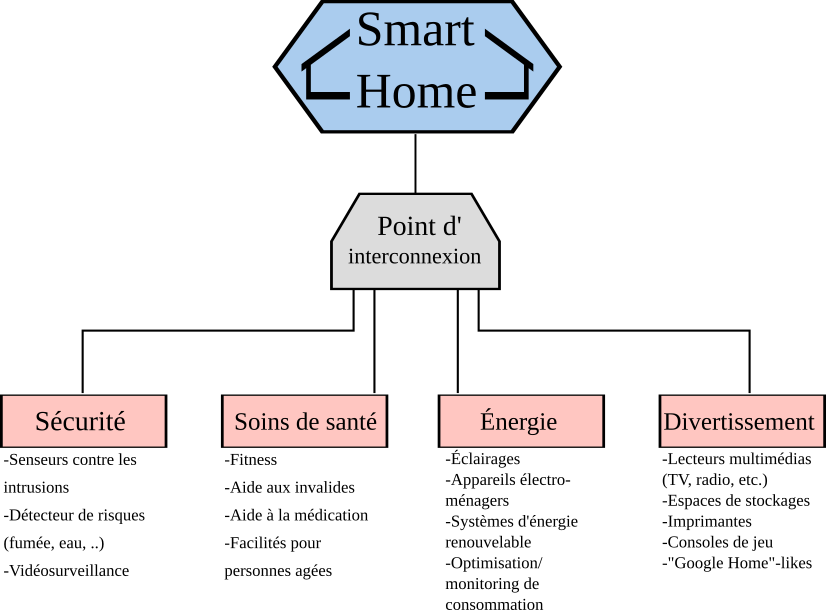
\includegraphics[scale=1.5]{smarthome_class.png}
\caption{Classification fonctionnelle des équipements \textit{IoT} d'une smarthome}
\label{sm_class}
\end{figure}

\newpage

\subsubsection{Exemples d'équipements}

La perception de ce qu'est l'\textit{IoT} par le grand public se résume énormément à l'environnement que constitue la \textit{smarthome} \cite{Berte2018}. Il s'agit d'une erreur d'incompréhension, on peut tenter de l'expliciter en analysant ce qui compose cette perception. La Figure~\ref{benef_SH} en donne une vision générale (tirée d'un sondage effectué aux États-Unis), qui va être étayée par les exemples concrets d'équipements la suivant.

\begin{figure}[!h]
\centering
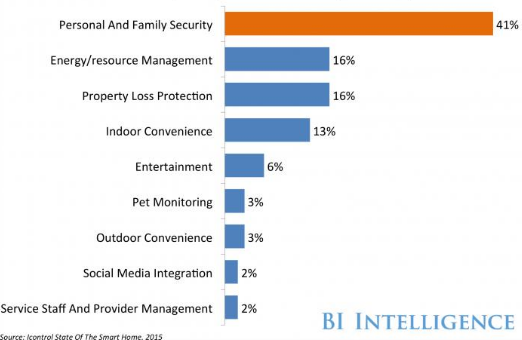
\includegraphics[scale=0.6]{benef_SH.png}
\caption{Top des meilleurs apports des \textit{smarthome} tel que perçu par les Américains}
\label{benef_SH}
\end{figure}

\vspace{0.3cm}

\minit{Appartenant à la classe sécurité}

\begin{itemize}
\item[$\bullet$] Caméras de vidéosurveillance dites IP
\item[$\bullet$] Systèmes de gestion d'alarme à distance
\item[$\bullet$] Verrous de portes intelligents
\item[$\bullet$] Simulateurs de présence et occupation du domicile
\end{itemize}
\vspace{0.3cm}
\minit{Appartenant à la classe soins de santé}

\begin{itemize}
\item[$\bullet$] Surveillance des patients à leur domicile (contrôle des mesures médicales)
\item[$\bullet$] Accessoires de fitness : montres, balances connectées et autres
\item[$\bullet$] Outils divers d'aide aux personnes invalides (fauteuils, bracelets de secours, ...)
\end{itemize}
\vspace{0.3cm}
\minit{Appartenant à la classe des énergies}

\begin{itemize}
\item[$\bullet$] Luminaires intelligents/automatisés contrôlables à distance
\item[$\bullet$] Frigos, lave-vaisselles, etc. 
\item[$\bullet$] Thermostats connectés, compteurs et senseurs énergétiques
\end{itemize}
\vspace{0.3cm}
\minit{Appartenant à la classe du divertissement \& multimédia}

\begin{itemize}
\item[$\bullet$] Outils de communication : smartphones, babyphones, etc.
\item[$\bullet$] SmartTV, consoles, casques connectés et lecteurs multimédia divers
\item[$\bullet$] Imprimantes et scanneurs en réseau
\item[$\bullet$] Assistants vocaux de maison comme le \textit{google home}
\end{itemize}
\newpage

\subsubsection{Restrictions des équipements}

Malgré le fait que l'ensemble des objets considérés comme appartenant à l'IoT soit très hétérogène, on peut distinguer plusieurs caractéristiques communes à beaucoup d'entre eux. Elles tendent généralement vers ce qui est vu comme une restriction par rapport à un ordinateur type classique (\textit{desktop}). Ces éléments constituent les plus gros freins au développement de la sécurité sur de tels système \cite{Wind2015}. Les conséquences de ces restrictions sont discutées plus en détail dans la section~\ref{prot_IoT} de ce document.\\

\minit{Conçus pour satisfaire une unique fonction}

Le meilleur exemple est celui des capteurs : un capteur a pour objectif de faire une mesure d'une grandeur physique (température, pression, etc.), d'en tirer une valeur numérique et de faire remonter par son interface avec le réseau cette information vers une unité centrale qui la traitera. Ce genre d'équipement est minimaliste au possible et ne peut donc pas remplir d'autre tâche.\\

\minit{Requièrent une faible consommation énergétique}

Les systèmes embarqués n'ont pas toujours accès à une source illimitée d'énergie, et auront donc une durée de vie limitée à celle de leur batterie. En conséquence, il est souhaitable d'économiser un maximum, ce qui peut se faire en réduisant les temps d'éveil de l'équipement et en optimisant le nombre d'opérations effectuées quand il tourne à plein régime. Dés lors, certains protocoles doivent être adapté et il peut également en résulter que l'aspect de la protection passer à la trappe.\\

\minit{Possèdent une interface réseau}

Le système doit avoir la capacité de communiquer les résultats obtenus pour la fonction qui lui est assignée. Il peut s'agit d'une transmission uni ou bi-directionnelle et en collaboration avec d'autres équipements IoT ou directement vers une machine centrale plus assimilable à un ordinateur. Le média peut également être filaire ou non, mais ce sera souvent le premier cas du fait que les équipements sont en général nombreux, petits et mobiles. À noter que cela rejoint la problématique de la consommation énergétique, alors grandement augmentée par les communications radios.\\ 

\minit{Sont codés à bas niveau}

Étant conçus pour ne remplir que des fonctions spécifiques, certains équipements ne sont pas programmables en utilisant des langages de haut niveau. Par conséquent, ce sont souvent des boites noires difficilement manipulable et statiques : aucune mise à jour ou patch n'est déployable aisément et les seules interactions que l'utilisateur peut avoir avec l'équipement sont celles prévues par l'interface de ce dernier s'il y en a une.


\newpage
\section{Présentations des pare-feus}

\subsection{Généralités}

\subsection{Types de pare-feu}

\subsection{Ressources logicielles importantes}

\newpage
\section{La protection dans l'\textit{IoT}}\label{prot_IoT}

\subsection{Vulnérabilités liées à l'\textit{IoT}}

\subsection{Possibilités d'amélioration}

\subsection{Solutions existantes}

\newpage
\section{Les pare-feus et l'\textit{IoT}}

\subsection{Différents types d'architecture}

\subsection{Les pare-feus domestiques}

\subsubsection{Caractéristiques d'un réseau domestique}

\subsubsection{Attaques possibles et conséquences}

\subsection{Application et implémentation}

\newpage

\section{Mise en pratique : ébauche}
\newpage
\section*{Conclusion}


\bibliographystyle{plain}
\bibliography{articles}

\end{document}